\chapter{Implementierung}

\section {Inbetriebnahme Greifarm}
Der OMX wird als Bausatz geliefert.Für die Inbetriebnahme ist daher der Zusammenbau und die Installation der entsprechenden Software  nötig. 
\subsection{Zusammenbau}
-Bausatz ca 40 Teile (ohne Schrauben)\\
-Rausbrechen Plastik bei Vorbereitung Servos\\
-Servos einzeln anschließen und per Dynamixel Wizard ID setzen\\
Der Bausatz des OMX besteht aus ca. 60 Teilen (ohne Schrauben, s. Abbildung \ref{fig:omxparts}).Einige der mit den Servomotoren mitgelieferten Teile werden dabei nicht benötigt, da der Bausatz des OMX diese auch enthält oder ersetzt (z.B. längere Kabel). Von allen Schrauben wurde außerdem Ersatz mitgeliefert.\\
Der Zusammenbau erfolgte nach der auf der Webseite verfügbaren Bauanleitung VERWEIS ANLEITUNG. Zu beachten ist, dass hier vorrausgesetzt wird, dass den Servos bereits die IDs 11 (Basis des Greifarms) bis 15 (Greifer) zugewiesen wurden. Dies kann über die Software DYNAMIXEL Wizard{\footnote{VERWEIS ODER LINK}} gemacht werden: die Servos einzeln über das U2D2{\footnote{ERKLÄRUNG ODER VERWEIS HINZUFÜGEN}} an den PC anschließen, die ID setzen und den Servo entsprechend markieren oder die ID merken. Weiterhin müssen bei den Abdeckungen der Servos 12 und 14 die vorgestanzten Abdeckungen herausgebrochen werden. Dies ist in der Anleitung leicht zu übersehen. Weiterhin wird angenommen, dass das Horn der Servos bereits angebracht ist. Hierbei ist darauf zu achten, dass die Einkerbung an Horn und Servo übereinstimmen.
\begin{figure}[h!]
\centering
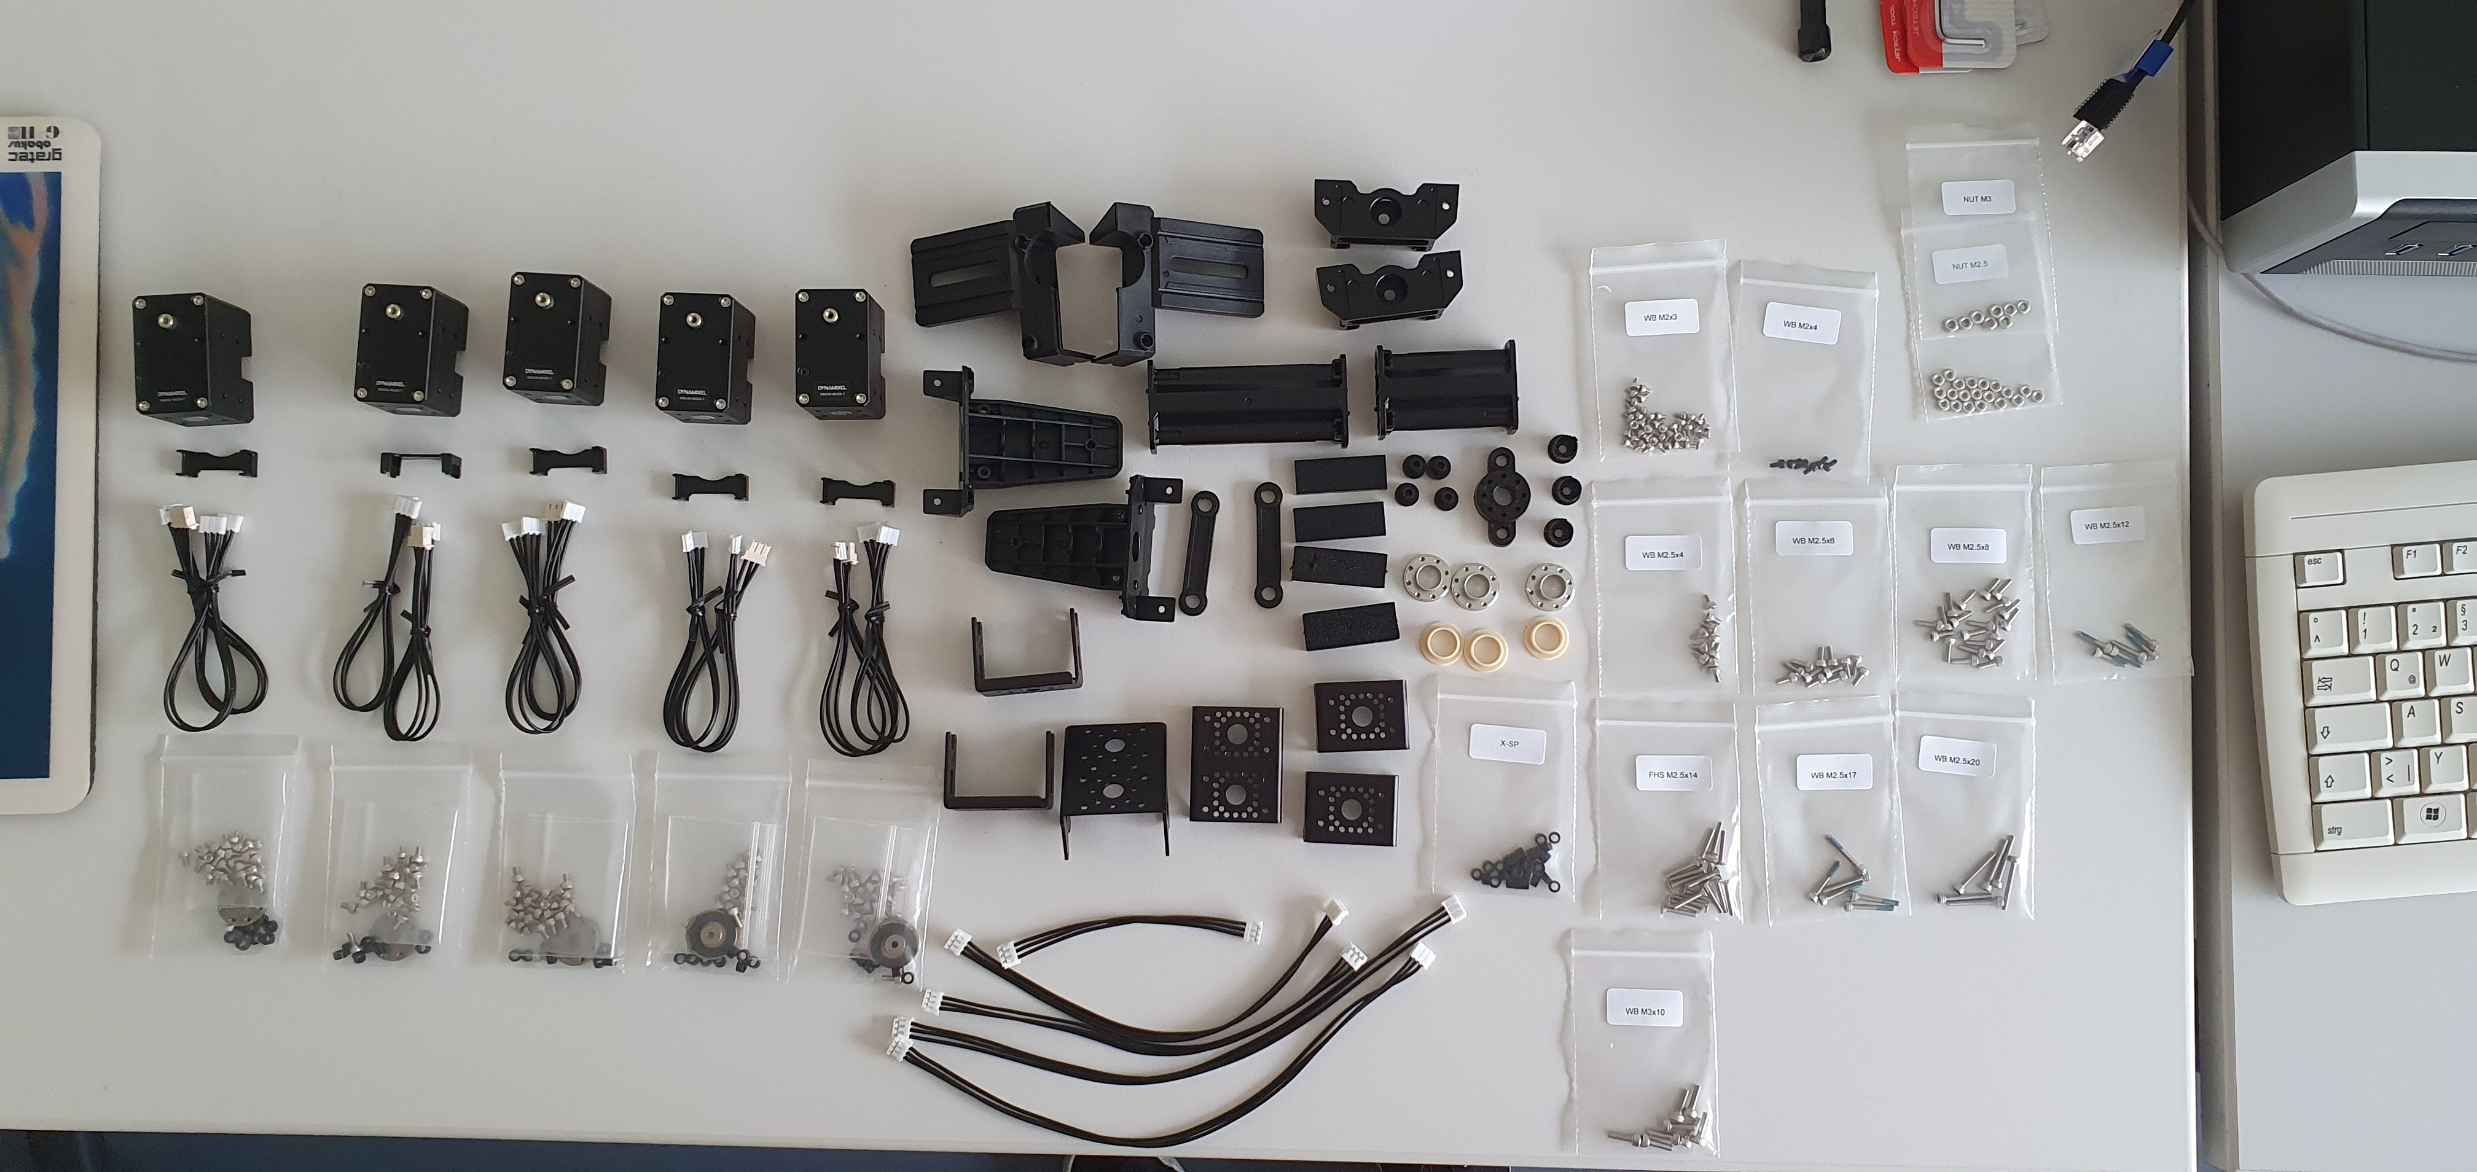
\includegraphics[width=\textwidth]{parts}
\caption{Bausatz für den OpenMANIPULATOR-X}
\label{fig:omxparts}
\end{figure}
\subsection{Virtuelle Maschine}
-Ubuntu 20.04\\
-- Auflösung Einstellung "keine"\\
-Installation ROS2 Foxy\\
-Installation OMX\\
Zur Nutzung des Greifarms wurde eine virtuelle Maschine (VM) mit VirtualBox {\footnote{https://www.virtualbox.org}} von Oracle aufgesetzt. Als Betriebssystem der VM wurde das für ROS2 Foxy empfohlene{\cite{foxyreq}} Ubuntu 20.04 {\footnote{https://releases.ubuntu.com/20.04/}} gewählt. Danach wurde entsprechend der Anleitung für den OpenMANIPULATOR-X {\cite{foxyinstall}} zuerst ROS 2 Foxy über das Installations-Script von ROBOTIS und im Anschluss die für den Greifarm benötigten Packages  installiert.
\section{Steuerung Greifarm}
\subsection{OMX-Controller}
\subsection{Topics}
\subsection{Kinematik}


\section{PlanSys2}
\subsection{PDDL-Domain}
-Durative Actions\\
-Gripper + Blockworld\\
- keine existential/negative Preconditions\\
\subsection{Action Nodes}

%\newpage